\documentclass[a4paper,12pt]{article} 

% First, we usually want to set the margins of our document. For this we use the package geometry.
\usepackage[top = 2.5cm, bottom = 2.5cm, left = 2.5cm, right = 2.5cm]{geometry} 
\usepackage[T1]{fontenc}
\usepackage[utf8]{inputenc}

% The following two packages - multirow and booktabs - are needed to create nice looking tables.
\usepackage{multirow} % Multirow is for tables with multiple rows within one cell.
\usepackage{booktabs} % For even nicer tables.

% As we usually want to include some plots (.pdf files) we need a package for that.
\usepackage{graphicx} 

% The default setting of LaTeX is to indent new paragraphs. This is useful for articles. But not really nice for homework problem sets. The following command sets the indent to 0.
% \usepackage{setspace}
% \setlength{\parindent}{0in}
\usepackage{indentfirst}

% Package to place figures where you want them.
\usepackage{float}

% The fancyhdr package let's us create nice headers.
\usepackage{fancyhdr}

\usepackage{amsmath,amsthm,tikz,minted,algorithm2e,ulem,amsfonts}
\usepackage[most]{tcolorbox}
\RestyleAlgo{ruled}
\usetikzlibrary{graphs, graphdrawing}
\usegdlibrary[trees]


% To make our document nice we want a header and number the pages in the footer.

\pagestyle{fancy} % With this command we can customize the header style.

\fancyhf{} % This makes sure we do not have other information in our header or footer.

\lhead{\footnotesize Artificial Intelligence(H): Final Review}% \lhead puts text in the top left corner. \footnotesize sets our font to a smaller size.

%\rhead works just like \lhead (you can also use \chead)
\rhead{\footnotesize Mengxuan Wu}

% Similar commands work for the footer (\lfoot, \cfoot and \rfoot).
% We want to put our page number in the center.
\cfoot{\footnotesize \thepage} 

\begin{document}

\newtcolorbox{tipsbox}{
  colback=yellow!20!white, % Background color
  colframe=blue!80!black,  % Border color
  fonttitle=\bfseries,     % Title font
  title=More Info,         % Box title
  breakable                % Make the box breakable
}

\newtcolorbox{warningbox}{
  colback=yellow!20!white, % Background color
  colframe=red!80!black,   % Border color
  fonttitle=\bfseries,     % Title font
  title=Easy to Mistake,   % Box title
  breakable                % Make the box breakable
}

\newtcolorbox{examplebox}{
  colback=yellow!20!white, % Background color
  colframe=green!75!black, % Border color
  fonttitle=\bfseries,     % Title font
  title=Example,           % Box title
  breakable                % Make the box breakable
}

\thispagestyle{empty} % This command disables the header on the first page. 

\begin{tabular}{p{15.5cm}}
{\large \bf Artificial Intelligence(H)} \\
Southern University of Science and Technology \\ Mengxuan Wu \\ 12212006 \\
\hline
\\
\end{tabular}

\vspace*{0.3cm} %add some vertical space in between the line and our title.

\begin{center}
	{\Large \bf Final Review}
	\vspace{2mm}

	{\bf Mengxuan Wu}
		
\end{center}  

\vspace{0.4cm}

\section{Intelligent Agents}

\subsection{Definition}

\paragraph{Agent} An \textbf{agent} is anything that can be viewed as perceiving its environment through sensors and acting upon that environment through actuators. An agent program runs in cycles of perceive, think, and act. An \textbf{agent function} is a mapping from percepts to actions. An agent is a combination of an architecture and a program, which should be complementary and compatible.

\paragraph{Rational Agent} For each possible percept sequence, a \textbf{rational agent} should select an action that is expected to maximize its performance measure, given the evidence provided by the percept sequence and whatever built-in knowledge the agent has.

\subsection{PEAS}

When we define a rational agent, we group the agent's performance elements into four categories: \textbf{Performance measure}, \textbf{Environment}, \textbf{Actuators}, and \textbf{Sensors}. This is called the PEAS description.

\begin{examplebox}
	For a self-driving car, the PEAS description is as follows:
	\begin{itemize}
		\item \textbf{Performance measure}: Safety, legality, passenger comfort, and arrival time.
		\item \textbf{Environment}: Roads, traffic, pedestrians, other cars, weather.
		\item \textbf{Actuators}: Steering wheel, accelerator, brake, signal lights, horn.
		\item \textbf{Sensors}: Cameras, LIDAR, GPS, speedometer, odometer, engine sensors.
	\end{itemize}
\end{examplebox}

\subsection{Properties of Environments}

\paragraph{Fully Observable vs. Partially Observable} An environment is \textbf{fully observable} if the agent's sensors give it access to the complete state of the environment at each point in time. Otherwise, the environment is \textbf{partially observable}.

\paragraph{Deterministic vs. Stochastic} If the next state of the environment is completely determined by the current state and the action executed by the agent, the environment is \textbf{deterministic}. Otherwise, the environment is \textbf{stochastic}.

\paragraph{Episodic vs. Sequential} The agent's experience is divided into episodes. Each episode consists of the agent perceiving and then acting. The choice of action in each episode depends only on the episode itself. In a \textbf{sequential} environment, the current decision could affect all future decisions.

\paragraph{Static vs. Dynamic} If the environment can change while an agent is deliberating (i.e., the environment does not wait for the agent to make a decision), the environment is \textbf{dynamic}. Otherwise, it is \textbf{static}.

\paragraph{Discrete vs. Continuous} A discrete environment has a finite number of percepts and actions. A continuous environment has a continuous range of percepts and actions.

\paragraph{Single-agent vs. Multi-agent} A single-agent environment contains exactly one agent. A multiagent environment contains multiple agents.

\paragraph{Known vs. Unknown} If the designer of the agent have knowledge of the environment, the environment is \textbf{known}. Otherwise, the environment is \textbf{unknown}.

\begin{examplebox}
  Consider the following environments:
  \begin{table}[H]
    \resizebox{\linewidth}{!}{
      \begin{tabular}{lccccc}
        \toprule
        \textbf{Environment} & \textbf{Observable} & \textbf{Deterministic} & \textbf{Agent} & \textbf{Static} & \textbf{Discrete} \\
        \midrule
        8-puzzle & Yes & Yes & Single-agent & Yes & Yes \\
        Chess & Yes & Yes & Multi-agent & Yes & Yes \\
        Poker & No & No & Multi-agent & Yes & Yes \\
        Car & No & No & Multi-agent & No & No \\
        \bottomrule
      \end{tabular}
    }
  \end{table}
\end{examplebox}

\subsection{Types of Agents}

\subsubsection{Simple Reflex Agents}

A \textbf{simple reflex agent} selects actions on the basis of the current percept, ignoring the rest of the percept history. It works well in fully observable, deterministic, and static environments with a few states.

Based on its definition, a simple reflex agent only works well in environments where the current percept is sufficient to determine the correct action. In other words, the environment must be fully observable.

\begin{figure}[H]
  \centering
  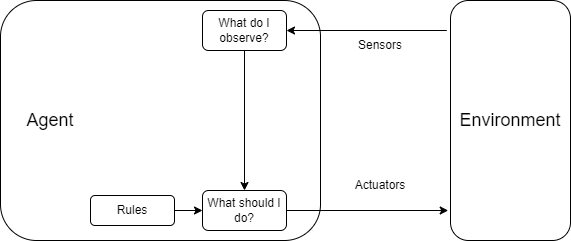
\includegraphics[width=0.6\textwidth]{figure/simple reflex.drawio.png}
  \caption{A simple reflex agent.}
\end{figure}

\begin{examplebox}
  Consider a simple reflex agent for a vacuum cleaner. The agent has two rules:
  \begin{itemize}
    \item If the current location is dirty, then clean.
    \item If the current location is clean, then move to the other location.
  \end{itemize}
  This agent works well in a fully observable, deterministic, and static environment with a few states.
\end{examplebox}

\subsubsection{Model-based Reflex Agents}

A \textbf{model-based reflex agent} maintains an internal state that depends on the percept history and thereby can handle partially observable environments. In other words, a model-based reflex agent learns how the world evolves over time, and uses this knowledge to predict the part of world that it cannot observe, thus making better decisions.

\begin{figure}[H]
  \centering
  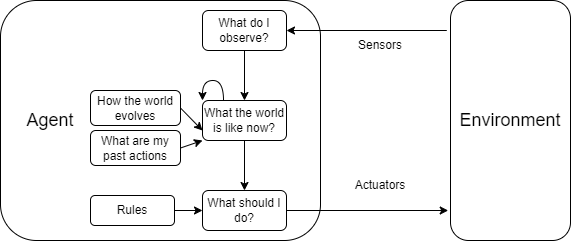
\includegraphics[width=0.6\textwidth]{figure/model based reflex.drawio.png}
  \caption{A model-based reflex agent.}
\end{figure}

\subsubsection{Goal-based Agents}

A \textbf{goal-based agent} is an agent that plans ahead to achieve its goals. It uses a \textbf{goal} to decide which action to take. And to do so, it must have the ability to predict the consequences of its actions.

\begin{figure}[H]
  \centering
  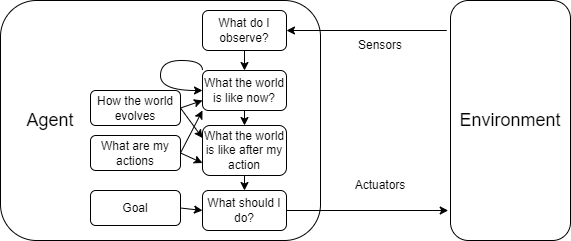
\includegraphics[width=0.6\textwidth]{figure/goal based.drawio.png}
  \caption{A goal-based agent.}
\end{figure}

\subsubsection{Utility-based Agents}

A \textbf{utility-based agent} is an agent that chooses the action that maximizes the expected utility of the agent's performance measure. It is similar to a goal-based agent, but it uses a \textbf{utility function} to decide which action to take.

\begin{figure}[H]
  \centering
  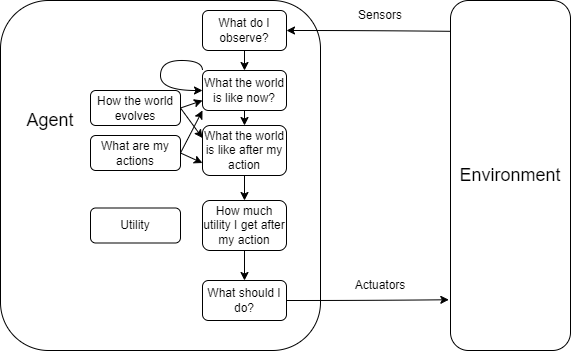
\includegraphics[width=0.6\textwidth]{figure/utility based.drawio.png}
  \caption{A utility-based agent.}
\end{figure}

\subsubsection{Learning Agents}

A \textbf{learning agent} is a generalized agent that can learn from its experience. It has 4 components: a \textbf{learning element} that is responsible for making improvements, a \textbf{performance element} that selects external actions, a \textbf{critic} that provides feedback on how well the agent is doing, and a \textbf{problem generator} that suggests actions that lead to new and informative experiences.

\subsection{Agent States}

\paragraph{Atomic Representation} An \textbf{atomic representation} assumes each state of the world is a black box without internal structure. For example, in a board game, each state is a unique configuration of the board.

\paragraph{Factored Representation} A \textbf{factored representation} decomposes the state into independent components. These variables can describe the complete state of the world. For example, in a gird-based world, the state can be decomposed into the position of the agent, positions of obstacles and goals, etc.

\paragraph{Structured Representation} A \textbf{structured representation} captures the relationships between components of the state. For example, a map that shows the distances between cities.

\section{Search}

\subsection{Problem Formulation}

\begin{itemize}
  \item \textbf{Initial state}: The state in which the agent starts.
  \item \textbf{States}: The set of all reachable states by any sequence of actions.
  \item \textbf{Actions}: The set of all possible actions that the agent can take.
  \item \textbf{Transition model}: A description of what each action does.
  \item \textbf{Goal test}: A function that determines whether a state is a goal state.
  \item \textbf{Path cost}: A function that assigns a numeric cost to each path.
\end{itemize}

\subsection{Search Space}

\paragraph{State Space vs. Search Space} The \textbf{state space} is the set of all states reachable from the initial state by any sequence of actions. The \textbf{search space} is an abstract configuration that models the sequence of actions taken by the agent. For example, a search tree is a search space, where its root is the initial state, branches are actions, and nodes result from applying actions to states.

A search space is divided into three parts: \textbf{frontier}, \textbf{explored set}, and \textbf{unexplored set}. The frontier is the set of nodes that have been generated but not yet expanded. The explored set is the set of nodes that have been expanded. The unexplored set is the set of nodes that have not been generated.

\subsection{Search Strategies}

Strategies are evaluated based on the following criteria: 
\begin{itemize}
  \item \textbf{Completeness}: Does the strategy guarantee to find a solution if one exists?
  \item \textbf{Optimality}: Does the strategy guarantee to find the optimal solution?
  \item \textbf{Time complexity}: How long does it take to find a solution?
  \item \textbf{Space complexity}: How much memory does it take to find a solution?
\end{itemize}

In particular, time complexity and space complexity are measured in terms of following factors:
\begin{itemize}
  \item \textbf{b}: The branching factor, i.e., the maximum number of children of any node.
  \item \textbf{d}: The depth of the solution.
  \item \textbf{m}: The maximum depth of the search tree.
\end{itemize}

We can classify search strategies into two categories: \textbf{uninformed search} and \textbf{informed search}.

\subsubsection{Uninformed Search}

\begin{itemize}
  \item \textbf{Breadth-first search (BFS)}: Expands the shallowest unexpanded node first.
  \item \textbf{Depth-first search (DFS)}: Expands the deepest unexpanded node first.
  \item \textbf{Depth-limited search (DLS)}: A variant of DFS that limits the depth of the search.
  \item \textbf{Iterative deepening search (IDS)}: A variant of DLS that gradually increases the depth limit.
  \item \textbf{Uniform-cost search (UCS)}: Expands the node with the lowest path cost (the same idea used in Dijkstra's algorithm).
\end{itemize}

Here are the properties of these strategies:
\begin{table}[H]
  \resizebox{\linewidth}{!}{
    \begin{tabular}{lcccc}
      \toprule
      \textbf{Strategy} & \textbf{Completeness} & \textbf{Optimality} & \textbf{Time complexity} & \textbf{Space complexity} \\
      \midrule
      BFS & Yes if $b$ is finite & Yes if cost is the same for every path & $O(b^d)$ & $O(b^d)$ \\
      DFS & Yes if the state space is finite & No & $O(b^m)$ & $O(bm)$ \\
      UCS & Yes if the solution has a finite cost & Yes & $O(b^{1 + \lfloor C^*/\epsilon \rfloor})$ & $O(b^{1 + \lfloor C^*/\epsilon \rfloor})$ \\
      \bottomrule
    \end{tabular}
  }
\end{table}
\textit{Note:} $C^*$ is the cost of the optimal solution, and $\epsilon$ is the minimum cost of any action.

\subsubsection{Informed Search}

\begin{itemize}
  \item \textbf{Greedy best-first search}: Expands the node that is closest to the goal.
  \item \textbf{A* search}: Expands the node that minimizes $f(n) = g(n) + h(n)$, where $g(n)$ is the cost to reach $n$ from the initial state, and $h(n)$ is the estimated cost to reach the goal from $n$.
  \item \textbf{IDA* search}: A variant of A* that uses iterative deepening.
\end{itemize}

The quality of informed search strategies depends on the quality of the heuristic function. 
\begin{itemize}
  \item \textbf{Admissible heuristic}: A heuristic function is admissible if it never overestimates the cost to reach the goal. In other words, $h(n) \leq h^*(n)$, where $h^*(n)$ is the true cost to reach the goal from $n$. An admissible heuristic guarantees to find the optimal solution.
  \item \textbf{Consistent heuristic}: A heuristic function is consistent if for every node $n$ and every successor $n'$ of $n$ generated by any action $a$, $h(n) \leq c(n, a, n') + h(n')$.
\end{itemize}

\begin{tipsbox}
  The closer the heuristic function is to the true cost, the more efficient the search strategy will be.
  \begin{itemize}
    \item If $h(n) = 0$, A* search degenerates into UCS.
    \item If $h(n) = h^*(n)$, we no longer need to find the distance by searching, since $h(n_{\text{start}})$ already gives the distance to the goal.
  \end{itemize}
\end{tipsbox}

\section{Local Search}

\subsection{Definition}

The search strategies we have discussed so far are called \textbf{systematic search}. For these strategies, when the goal is reached, a solution that consists of a sequence of actions is found. 

However, sometimes we do not need to know how to reach the goal (i.e., the sequence of actions). Instead, we only need to know the state that satisfies the goal. In this case, we can use \textbf{local search}.

\begin{examplebox}
  AI training is a good example of local search. All we care about is the final model that has the best performance. We do not need to know how the model is trained.
\end{examplebox}

The basic idea of local search is to keep a few states in memory and iteratively improve them. This means we only longer need to store the entire search tree, which saves memory.

Although local search is not guaranteed to find the optimal solution, it often can find a good solution in a reasonable amount of time.

\subsection{Local Search Strategies}

\subsubsection{Hill Climbing}

\textbf{Hill climbing} is a simple local search strategy that iteratively improves the current state by moving to the neighboring state with the highest value. However, this might cause the agent to get stuck in a local maximum or a plateau.

Some variants of hill climbing include:
\begin{itemize}
  \item \textbf{Sideways move}: Allow the agent to move to a neighboring state with the same value. This allows the agent to escape plateaus, but not local maxima.
  \item \textbf{Random-restart hill climbing}: Restart the search from a random state.
  \item \textbf{Stochastic hill climbing}: Randomly select the next state among the neighboring states.
  \item \textbf{Local beam search}: Keep $k$ states in memory and expand them simultaneously.
  \item \textbf{Stochastic beam search}: Randomly select $k$ states among the neighboring states.
\end{itemize}

\subsubsection{Simulated Annealing}

\textbf{Simulated annealing} is a variant of hill climbing that allows the agent to move to a neighboring state with a lower value with a certain probability. This probability decreases over time. This allows the agent to escape local maxima.

The probability of moving to a neighboring state with a lower value is given by:
\begin{equation*}
  P(\text{move to } n') = \begin{cases}
    1 & \text{if } \Delta E < 0 \\
    e^{-\frac{\Delta E}{T}} & \text{otherwise}
  \end{cases}
\end{equation*}
where $\Delta E = V(n) - V(n')$ is the difference in value between the current state and the neighboring state, and $T$ is the temperature.

\subsubsection{Genetic Algorithms}

\textbf{Genetic algorithms} is a variant of stochastic beam search. It is inspired by the process of natural selection. The algorithm maintains a population of states. Successor states are generated by combining two parent states. The algorithm then selects a new population by evaluating the fitness of each state.

The major improvement of genetic algorithms is that produce new states by combining two parent states, not by modifying a single state. This allows the algorithm to explore a larger search space.

\subsection{Better Heuristics*}

\subsubsection{Dominance}

The quality of local search strategies depends on the quality of the heuristic function. In the previous section, we discussed the admissible and consistent heuristic functions. However, only looking at these two properties is not enough, because we can easily find many admissible and consistent heuristic functions. To compare different admissible heuristic functions, we consider \textbf{dominance}.

We say that a heuristic function $h_1$ \textbf{dominates} another heuristic function $h_2$ if $h_1(n) \geq h_2(n)$ for all nodes $n$. In other words, $h_1$ is better than $h_2$ if $h_1$ is always greater than or equal to $h_2$.

\begin{tipsbox}
  From a collection of admissible heuristic functions $h_1, h_2, \ldots, h_n$, we can construct a new heuristic function $h(n) = \max\{h_1(n), h_2(n), \ldots, h_n(n)\}$. It is easy to see that $h$ dominates all $h_i$.
\end{tipsbox}

\subsubsection{Methods to Find Good Heuristics}

\begin{itemize}
  \item \textbf{Relaxation}: Relax the problem by removing constraints. For example, in the 8-puzzle, we can relax the constraint that a tile can only move to adjacent empty cells, and allow it to move to any empty cell. Or we can relax the constraint that a tile can move to an occupied cell.
  \item \textbf{Generated from sub-problems}: Only solve a part of the problem, and use the cost of the solution as the heuristic function. For example, in the 8-puzzle, we can solve the problem for half of the tiles, and use the cost of the solution as the heuristic function.
  \item \textbf{Generated from experience}: Use the cost of the solution of similar problems as the heuristic function. For example, in the 8-puzzle, we can use the cost of the solution of similar 8-puzzles as the heuristic function.
\end{itemize}

\section{Adversarial Search}

In Adversarial Search, we have an additional utility function that assigns a numeric value to each terminal state for each player. The goal of each player is to maximize its utility. If the sum of the utilities of all players is 0, the game is called a \textbf{zero-sum game}.

\subsection{Minimax Algorithm}

The \textbf{minimax algorithm} is a search algorithm that is used to find the optimal strategy for a player in a two-player zero-sum game. The algorithm is based on the following idea: if both players play optimally, each player will choose the action that maximizes his utility, and assume that the opponent will choose the action that minimizes his utility (to be noticed that here two ``his'' represent the same player).

For a state $s$, $minimax(s)$ is:
\begin{equation*}
  \text{minimax}(s) = \begin{cases}
    \text{utility}(s) & \text{if } \text{terminal}(s) \\
    \max_{a \in \text{actions}(s)} \text{minimax}(\text{result}(s, a)) & \text{if } \text{player}(s) = \text{MAX} \\
    \min_{a \in \text{actions}(s)} \text{minimax}(\text{result}(s, a)) & \text{if } \text{player}(s) = \text{MIN}
  \end{cases}
\end{equation*}
which represents the maximum utility that can be obtained from state $s$.

\begin{figure}[H]
  \centering
  \begin{tikzpicture}[binary tree layout, nodes={draw, circle, minimum size=0.8cm}]
    \node [fill = red!50!white] {7}
      child{node[fill = blue!50!white]{7}
        child{node[fill = red!50!white]{9}
          child{node[fill = blue!50!white]{2}}
          child{node[fill = blue!50!white]{9}}
        }
        child{node[fill = red!50!white]{7}
          child{node[fill = blue!50!white]{7}}
          child{node[fill = blue!50!white]{4}}
        }
      }
      child{node[fill = blue!50!white]{5}
        child{node[fill = red!50!white]{9}
          child{node[fill = blue!50!white]{8}}
          child{node[fill = blue!50!white]{9}}
        }
        child{node[fill = red!50!white]{5}
          child{node[fill = blue!50!white]{3}}
          child{node[fill = blue!50!white]{5}}
        }
      };
  \end{tikzpicture}
  \caption{An example of the minimax algorithm, where the red nodes represent the MAX player, and the blue nodes represent the MIN player.}
\end{figure}

We can observe that the tree is build bottom-up. The algorithm starts from the terminal states and propagates the utility values up to the root. 

However, it is not practical to search the entire game tree. And some techniques can be used to improve the performance of the minimax algorithm.

\subsubsection{Alpha-Beta Pruning}

\textbf{Alpha-beta pruning} is a technique that reduces the number of nodes that need to be evaluated in the minimax algorithm. The idea is that, since the MAX player will choose the maximum value among the children, if we know the value of certain subtree will never be the maximum value, then we do not need to explore it, and same for the MIN player.

For example, below displays an incomplete DFS search tree, where the black nodes are pruned.
\begin{figure}[H]
  \centering
  \begin{tikzpicture}[tree layout, nodes={draw, circle, minimum size=1.5cm}]
    \node [fill = red!50!white] {$r \geq 3$}
      child{node[fill = blue!50!white]{$v_1 = 3$}
        child{node[fill = red!50!white]{$v_{11} = 3$}}
        child{node[fill = red!50!white]{$v_{12} = 9$}}
        child{node[fill = red!50!white]{$v_{13} = 8$}}
      }
      child{node[fill = blue!50!white]{$v_2 \leq 2$}
        child{node[fill = red!50!white]{$v_{21} = 2$}}
        child{node[fill = black]{}}
        child{node[fill = black]{}}
      }
      child{node[fill = blue!50!white]{}
        child{node[fill = red!50!white]{}}
        child{node[fill = red!50!white]{}}
        child{node[fill = red!50!white]{}}
      };
  \end{tikzpicture}
\end{figure}

In this example, we discovered that $v_{21} = 2$. Since MIN player decide on the value of $v_2$, he will choose the smallest value among $v_{21}$, $v_{22}$, and $v_{23}$. Since $v_{21} = 2$, the value of $v_2$ will never be greater than 2. Then, when MAX player decide on the value of $r$, he will choose the largest value among $v_1$, $v_2$ and $v_3$. Since $v_2 \leq 2$ and $v_1 = 3$, he will never choose $v_2$. Therefore, we can prune the subtree rooted at $v_2$.

\begin{tipsbox}
  Formally, $minimax(r)$ is:
  \begin{align*}
    \text{minimax}(r) &= \max\{\min\{3, 9, 8\}, \min\{2, x, y\}, \ldots\} \\
    &= \max\{3, \min\{2, x, y\}, \ldots\}
  \end{align*}

  Obviously, the value of $\min\{2, x, y\}$ can never be greater than 3. Therefore, we can prune the subtree rooted at $v_2$.
\end{tipsbox}

Based on this idea, we can define $\alpha$ as the best value that the MAX player has found so far at any choice point along the path for MAX, and $\beta$ as the best value that the MIN player has found so far at any choice point along the path for MIN. Then, we can prune the subtree rooted at a node $n$ if $\text{minimax}(n) \leq \alpha$ for MIN player, or $\text{minimax}(n) \geq \beta$ for MAX player.

Here is the pseudocode for the alpha-beta pruning algorithm:
\begin{minted}{python}
def alphabeta_search(game, state):
  player = state.to_move

  def max_value(state, alpha, beta):
      if game.is_terminal(state):
          return game.utility(state, player), None
      v, move = -infinity, None
      for a in game.actions(state):
          v2, _ = min_value(game.result(state, a), alpha, beta)
          if v2 > v:
              v, move = v2, a
          if v >= beta:
              return v, move
          alpha = max(alpha, v)
          
      return v, move

  def min_value(state, alpha, beta):
      if game.is_terminal(state):
          return game.utility(state, player), None
      v, move = infinity, None
      for a in game.actions(state):
          v2, _ = max_value(game.result(state, a), alpha, beta)
          if v2 < v:
              v, move = v2, a
          if v <= alpha:
              return v, move
          beta = min(beta, v)
          
      return v, move

  return max_value(state, -infinity, +infinity)
\end{minted}

\subsubsection{Move Ordering}

From the process of alpha-beta pruning, we can see that the order of the children of a node is important. If we can find a good ordering, we can prune more nodes. 

The ordering of the children of a node is often done by heuristic function, which evaluate the value of each child. For example, an Othello agent can use the difference in the number of pieces as the heuristic function.

\subsubsection{Early Cutoffs}

Since utility function only provides scores for terminal states, the algorithm must reach the terminal states to evaluate, which is time-consuming. We can use early cutoffs to stop the search early. For example, we find an evaluation function that can estimate the value of a non-terminal state, thus we stop at any moment and use the stated examined so far to decide the best move.

With this technique, we can use iterative deepening, where we gradually increase the depth of the search. This allows us to find a good move in a reasonable amount of time, or to stop the search early if we run out of time.

\subsection{Stochastic Games}

Stochastic games may include randomness, for example in the form of dice rolls. In this case, we can use the \textbf{expectiminimax algorithm}, which add a new type of node called \textbf{chance node} to the game tree. The value of a chance node is the expected value of its children.

For a state $s$, $expectiminimax(s)$ is:

\begin{equation*}
  \resizebox{\linewidth}{!}{
    $\text{expectiminimax}(s) = \begin{cases}
      \text{utility}(s) & \text{if } \text{terminal}(s) \\
      \max_{a \in \text{actions}(s)} \text{expectiminimax}(\text{result}(s, a)) & \text{if } \text{player}(s) = \text{MAX} \\
      \min_{a \in \text{actions}(s)} \text{expectiminimax}(\text{result}(s, a)) & \text{if } \text{player}(s) = \text{MIN} \\
      \sum_{a \in \text{actions}(s)} \text{probability}(a) \times \text{expectiminimax}(\text{result}(s, a)) & \text{if } \text{player}(s) = \text{CHANCE}
    \end{cases}$
  }
\end{equation*}

\section{Constraint Satisfaction Problems}

For a constraint satisfaction problem (CSP), each state is defined by a set of variables $X$ (factored representation), each of which has a domain of possible values $D$, and a set of constraints $C$ that specify allowable combinations of values for subsets of variables (unary, binary, global, and soft constraints).

The goal of a CSP is to find an assignment of values to variables that satisfies all constraints. A solution to a CSP is called a \textbf{consistent assignment}.

\subsection{Backtracking Search}

\textbf{Backtracking search} is a variant of depth-first search that is used to solve CSPs. The major difference is that backtracking search can use inference to reduce the search space.

The algorithm works as follows:
\begin{enumerate}
  \item Select an unassigned variable.
  \item Select a value from the domain of the variable, and assign it to the variable.
  \item If the assignment is consistent with the constraints, recursively assign values to the remaining variables. Otherwise, backtrack.
\end{enumerate}

Several techniques can be used to improve the performance of backtracking search:
\begin{itemize}
  \item \textbf{Minimum remaining values (MRV)}: When selecting an unassigned variable, choose the variable with the fewest remaining values in its domain.
  \item \textbf{Least constraining value (LCV)}: When selecting a value for a variable, choose the value that rules out the fewest values in the remaining variables.
  \item \textbf{Forward checking}: When assigning a value to a variable, check if the remaining variables have any values left in their domains. If not, backtrack.
\end{itemize}

\subsection{Types of Consistency}

\paragraph{Node consistency} A variable is node consistent if every value in its domain satisfies the variable's unary constraints.

\paragraph{Arc consistency} $X \to Y$ is arc consistent if for every value $x$ in the domain of $X$, there is some value $y$ in the domain of $Y$ that satisfies the binary constraint between $X$ and $Y$.

\paragraph{Path consistency} Generalize arc-consistency for multiple constraints. This is not important because it is always possible to transform all global constraints into binary constraints.

\subsubsection{AC-3 Algorithm}

The \textbf{AC-3 algorithm} checks whether a CSP is arc consistent. The algorithm works as follows:

\begin{algorithm}[H]
  \caption{AC-3 algorithm}
  \KwIn{A CSP $X$, a set of variables $V$, and a set of constraints $C$}
  \KwOut{Whether the CSP is arc consistent}
  Initialize a queue $Q$ with all arcs in $C$\;
  \While{$Q$ is not empty}{
    Remove the first arc $(X_i, X_j)$ from $Q$\;
    \If{REVISE$(X_i, X_j)$}{
      \If{$D_i = \emptyset$}{
        \Return \textbf{false}\;
      }
      \For{each $X_k$ such that $X_k$ is a neighbor of $X_i$ and $X_k \neq X_j$}{
        Add $(X_k, X_i)$ to $Q$\;
      }
    }
  }
\end{algorithm}

\begin{algorithm}[H]
  \caption{REVISE$(X_i, X_j)$}
  \KwIn{Two variables $X_i$ and $X_j$}
  \KwOut{Whether the domain of $X_i$ is revised}
  $revised \gets \textbf{false}$\;
  \For{each value $x$ in $D_i$}{
    \If{no value $y$ in $D_j$ allows $(x, y)$ to satisfy the constraint between $X_i$ and $X_j$}{
      Remove $x$ from $D_i$\;
      $revised \gets \textbf{true}$\;
    }
  }
  \Return $revised$\;
\end{algorithm}

The idea of the AC-3 algorithm is that:
\begin{enumerate}
  \item Build a queue for arcs that need to be checked.
  \item Check each arc in the queue. Modify the domain of the first variable until it is arc consistent with the second variable.
  \item If the domain of the first variable is empty, the CSP is not arc consistent (no valid assignment for the first variable).
  \item Since we modified the domain of the first variable, this may cause some arcs to be inconsistent. Add these arcs to the queue.
\end{enumerate}

The time complexity of the AC-3 algorithm is $O(n^2d^3)$, where $n$ is the number of variables and $d$ is the maximum domain size.

\section{Logic}

\subsection{Entailment and Inference}

\paragraph{Entailment} A sentence $KB \models \alpha$ means that $\alpha$ is true in all models where $KB$ is true. In other words, $\alpha$ is entailed by $KB$.

\paragraph{Inference} Inference is the process of deriving new sentences from existing sentences. It applies rules of inference to $KB$ to build a new sentence $\alpha$. Inference is denoted as $KB \vdash \alpha$.

Entailment enumerates all possible models of $KB$ to check if $\alpha$ is true in all models, while inference does not.

\subsection{Sound and Complete}

An inference algorithm we desire should be sound and complete. A sound algorithm is one that never infer a false sentence from a true sentence, while a complete algorithm is one that can infer all true sentences. In other words, a sound and complete algorithm is one that can infer all and only true sentences.

With inference rules, we can guarantee the soundness of algorithm. To achieve completeness, we use resolution or forward/backward chaining.

\subsubsection{Resolution}

The resolution law can be written as:
\begin{equation*}
  \frac{p_1 \lor p_2 \lor \ldots \lor p_n, \neg q_1 \lor \neg q_2 \lor \ldots \lor \neg q_m}{p_1 \lor p_2 \lor \ldots \lor p_{i-1} \lor p_{i+1} \lor \ldots \lor p_n \lor q_1 \lor q_2 \lor \ldots \lor q_{j-1} \lor q_{j+1} \lor \ldots \lor q_m}
\end{equation*}
where $p_i$ and $q_j$ are complementary literals.

\subsubsection{Forward and Backward Chaining}

\paragraph{Forward Chaining} Forward chaining is a simple inference algorithm that starts with the known facts and repeatedly applies Modus Ponens to Horn Clauses and add result back to $KB$.

\paragraph{Backward Chaining} Backward chaining is goal-driven. It repeatedly checks the premise of target clause. This gives linear complexity in size of $KB$.

\section{Machine Learning}

\subsection{Supervised vs. Unsupervised Learning}

\paragraph{Supervised Learning} In supervised learning, the algorithm learns from labeled data, where each example is a pair of input and output. The goal is to learn a function that maps inputs to outputs. Within supervised learning, we have two types of tasks: \textbf{classification} (discrete output) and \textbf{regression} (continuous output).

\paragraph{Unsupervised Learning} In unsupervised learning, the algorithm learns from unlabeled data. The goal is to find hidden patterns in the data.

\subsubsection{Example: K-Nearest Neighbors}

The k-nearest neighbors (KNN) is a simple supervised learning algorithm that can be used for both classification and regression. Although most ML algorithms build a model from the training data, KNN algorithm is an exception.

The core idea of the KNN algorithm that two data points are similar if they are close to each other, and two similar data points should have the same label. The algorithm works as follows:
\begin{itemize}
  \item \textbf{Train} Add all data points to the training set.
  \item \textbf{Predict}
    \begin{enumerate}
      \item For a new data point, calculate the distance between the new data point and all data points in the training set. For this step, we can use Euclidean distance, Manhattan distance, etc.
      \item Select the $k$ nearest data points.
        \begin{itemize}
          \item For classification, return the most common label among the $k$ nearest data points.
          \item For regression, return the average value of the $k$ nearest data points.
        \end{itemize}
    \end{enumerate}
\end{itemize}

The pros and cons of KNN are:
\begin{itemize}
  \item Pros
    \begin{itemize}
      \item Simple
      \item No training phase
      \item No model or hyperparameters, no assumptions about the data
    \end{itemize}
  \item Cons
    \begin{itemize}
      \item Slow prediction phase ($O(nd)$, where $n$ is the number of data points and $d$ is the number of features)
      \item Require large dataset
      \item Sensitive to the distance metric
      \item Suffers from the curse of dimensionality
    \end{itemize}
\end{itemize}

\subsection{Train, Validate and Test}

\subsubsection{Loss Function}

To evaluate the performance of a model, we need a loss function that measures the difference between the predicted value and the true value. Different tasks require different loss functions.

For classification tasks, we often use the cross-entropy loss, which is defined as:
\begin{equation*}
  \text{Cross-entropy loss} = -\sum_{i=1}^{n} y_i \log(p_i)
\end{equation*}
where $y_i$ is the true label in one-hot encoding, and $p_i$ is the predicted probability.

For regression tasks, we often use the mean squared error (MSE), which is defined as:
\begin{equation*}
  \text{MSE} = \frac{1}{2n} \sum_{i=1}^{n} (y_i - \hat{y}_i)^2
\end{equation*}

\subsubsection{Structural Risk Minimization}

\begin{figure}[H]
  \centering
  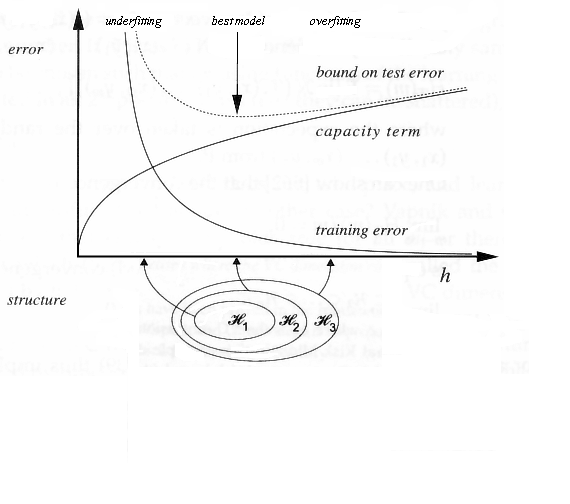
\includegraphics[width=0.6\textwidth]{figure/Sewell2006.png}
  \caption{Overfitting and underfitting.}
\end{figure}

When we train a model, we want to find a balance between underfitting and overfitting. Underfitting occurs when the model is too simple to capture the underlying pattern in the data, while overfitting occurs when the model is too complex and captures noise in the data.

Underfitting is featured by high bias and low variance, with high training error and high test error. Overfitting is featured by low bias and high variance, with low training error and high test error.

To avoid overfitting, here are some techniques:
\begin{itemize}
  \item \textbf{Feature selection}: Remove irrelevant features.
  \item \textbf{Regularization}: Add a penalty term to the loss function.
  \item \textbf{Cross-validation}: Estimate the test error with a validation set.
  \item \textbf{Model selection}: Choose a simpler model (lower degree polynomial, smaller neural network, etc.).
\end{itemize}

\subsubsection{K-Fold Cross-Validation}

K-fold cross-validation is a technique that estimates the test error by splitting the training set into $k$ folds. The algorithm works as follows:
\begin{enumerate}
  \item Randomly partition the training set $D$ into $k$ equal-sized subsets, denoted as $D_1, D_2, \ldots, D_k$.
  \item For $i = 1, 2, \ldots, k$, train the model on $D - D_i$ and evaluate the model on $D_i$.
  \item Calculate the average test error.
\end{enumerate}

\subsubsection{Confusion Matrix}

A confusion matrix is a table that is often used to describe the performance of a classification model. An example of a confusion matrix is shown below:
\begin{table}[H]
  \centering
  \begin{tabular}{lcc}
    \toprule
    & \textbf{Predicted Positive} & \textbf{Predicted Negative} \\
    \midrule
    \textbf{Actual Positive} & True Positive (TP) & False Negative (FN) \\
    \textbf{Actual Negative} & False Positive (FP) & True Negative (TN) \\
    \bottomrule
  \end{tabular}
\end{table}

Some common metrics that can be calculated from a confusion matrix include:
\begin{itemize}
  \item \textbf{Accuracy}: $\frac{TP + TN}{TP + FP + FN + TN}$, the proportion of correct predictions.
  \item \textbf{Precision}: $\frac{TP}{TP + FP}$, the proportion of positive predictions that are correct.
  \item \textbf{Recall}: $\frac{TP}{TP + FN}$, the proportion of actual positives that are correctly predicted.
  \item \textbf{F1 score}: $2 \times \frac{\text{Precision} \times \text{Recall}}{\text{Precision} + \text{Recall}}$, the harmonic mean of precision and recall.
\end{itemize}

\section{Regression}

\subsection{Linear Regression}

A linear regression model is a linear model (i.e., the output is a linear combination of the input features) that is used to predict a continuous value. The model is defined as:
\begin{equation*}
  y = w_0 + \sum_{i=1}^{d} w_i x_i
\end{equation*}
where $y$ is the predicted value, $w_0$ is the bias term, $w_i$ are the weights, $x_i$ are the input features, and $d$ is the dimension of the input features.

The goal of linear regression is to find the weights that minimize the mean squared error (MSE) between the predicted value and the true value. The loss function is defined as:
\begin{equation*}
  \text{MSE} = \frac{1}{2n} \sum_{i=1}^{n} (y_i - \hat{y}_i)^2
\end{equation*}
where $y_i$ is the true value, $\hat{y}_i$ is the predicted value, and $n$ is the number of data points.

\subsubsection{Normal Equation}

Let $\mathbf{X} = \begin{bmatrix} 1 & x_{11} & x_{12} & \ldots & x_{1d} \\ 1 & x_{21} & x_{22} & \ldots & x_{2d} \\ \vdots & \vdots & \vdots & \ddots & \vdots \\ 1 & x_{n1} & x_{n2} & \ldots & x_{nd} \end{bmatrix}$, $\mathbf{y} = \begin{bmatrix} y_1 \\ y_2 \\ \vdots \\ y_n \end{bmatrix}$, and $\mathbf{w} = \begin{bmatrix} w_0 \\ w_1 \\ w_2 \\ \vdots \\ w_d \end{bmatrix}$.

Then the loss function can be written as:
\begin{equation*}
  \text{MSE} = \frac{1}{2n} (\mathbf{y} - \mathbf{X} \mathbf{w})^T (\mathbf{y} - \mathbf{X} \mathbf{w})
\end{equation*}

The unique solution to the normal equation $\frac{\partial \text{MSE}}{\partial \mathbf{w}} = 0$ is:
\begin{equation*}
  \mathbf{w} = (\mathbf{X}^T \mathbf{X})^{-1} \mathbf{X}^T \mathbf{y}
\end{equation*}

However, the normal equation has some limitations:
\begin{itemize}
  \item We cannot guarantee that $(\mathbf{X}^T \mathbf{X})^{-1}$ exists. In some extreme cases (for example, when $d > n$), we can prove that $(\mathbf{X}^T \mathbf{X})^{-1}$ does not exist.
  \item Even if $(\mathbf{X}^T \mathbf{X})^{-1}$ exists, the time complexity for matrix inversion is $O(d^3)$, which is not efficient for large $d$.
  \item Due to its linear nature, the normal equation cannot capture non-linear relationships between the input features and the output.
\end{itemize}

\subsubsection{Gradient Descent}

Gradient descent is an iterative optimization algorithm that is used to find the weights that minimize the loss function. The algorithm works as follows:
\begin{enumerate}
  \item Initialize the weights $\mathbf{w}$ randomly.
  \item Calculate the gradient of the loss function with respect to the weights: $\frac{\partial \text{MSE}}{\partial \mathbf{w}}$.
  \item Update the weights: $\mathbf{w} \gets \mathbf{w} - \alpha \frac{\partial \text{MSE}}{\partial \mathbf{w}}$, where $\alpha$ is the learning rate.
  \item Repeat steps 2 and 3 until the weights converge.
\end{enumerate}

\begin{examplebox}
  For a first order linear regression model defined as:
  \begin{equation*}
    y = w_0 + w_1 x
  \end{equation*}
  the update rule for gradient descent is:
  \begin{align*}
    w_0 &\gets w_0 - \alpha \frac{1}{n} \sum_{i=1}^{n} (w_0 + w_1 x_i - y_i) \\
    w_1 &\gets w_1 - \alpha \frac{1}{n} \sum_{i=1}^{n} (w_0 + w_1 x_i - y_i) x_i
  \end{align*}
\end{examplebox}

\subsection{Logistic Regression}

Logistic regression is a linear model that is used to predict the probability of a binary outcome. The model is defined as:
\begin{equation*}
  y = \sigma(w_0 + \sum_{i=1}^{d} w_i x_i)
\end{equation*}
where $\sigma(z) = \frac{1}{1 + e^{-z}}$ is the sigmoid function.

The loss function for logistic regression is the cross-entropy loss, which is defined as:
\begin{equation*}
  \text{Cross-entropy loss} = -\frac{1}{n} \sum_{i=1}^{n} y_i \log(p_i) + (1 - y_i) \log(1 - p_i)
\end{equation*}

\section{Support Vector Machine}

A support vector machine (SVM) is a supervised learning algorithm that is used for classification tasks. The goal of an SVM is to find the hyperplane that separates the data points of different classes with the maximum margin.

\subsection{Linear SVM}

One challenge met by linear regression is that many hyperplanes can separate the data points, but which one is the best? SVM solves this problem. The core idea of linear SVM is to find a hyperplane that its minimum distance to any data point is maximized. Although the idea looks simple, the mathematical formulation of the problem is complex, however beautiful.

A linear SVM is a linear model that is defined as:
\begin{equation*}
  y = \text{sign}\left(b + \sum_{i=1}^{d} w_i x_i\right)
\end{equation*}
where sign is the sign function, defined as:
\begin{equation*}
  \text{sign}(z) = \begin{cases}
    1 & \text{if } z \geq 0 \\
    -1 & \text{otherwise}
  \end{cases}
\end{equation*}

The decision boundary of an SVM is defined as:
\begin{equation*}
  b + \sum_{i=1}^{d} w_i x_i = 0
\end{equation*}

Since we have a decision boundary, we can find the minimum distance $c$ between the decision boundary and the closest data point. This distance is called the margin. Now we define the plus-plane as $b + \sum_{i=1}^{d} w_i x_i \geq c$ and the minus-plane as $b + \sum_{i=1}^{d} w_i x_i \leq -c$. For any point, its distance to the decision boundary is at least $c$.

To simplify the problem, we can scale the weights and the bias term by $c$ (i.e., $w_i \gets \frac{w_i}{c}$ and $b \gets \frac{b}{c}$). Now the plus-plane becomes $b + \sum_{i=1}^{d} w_i x_i \geq 1$ and the minus-plane becomes $b + \sum_{i=1}^{d} w_i x_i \leq -1$. For any point, its distance to the decision boundary is at least 1.

Finally, we can define the margin as the distance between the plus-plane and the minus-plane, which is $\frac{2}{\|w\|}$. Any data point that is on the plus-plane or the minus-plane is called a support vector.

\begin{figure}[H]
  \centering
  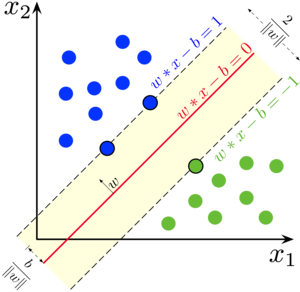
\includegraphics[width=0.6\textwidth]{figure/SVM_margin.png}
  \caption{The margin of an SVM.}  
\end{figure}

The goal of an SVM is to maximize the margin. This has a clear interpretation: the larger the margin, the more separation between the classes.

Now, if we skip the derivation, we can find that the optimization problem of an SVM can be simply written as:
\begin{equation*}
  \min_{w, b} \frac{1}{2} \|w\|^2 \quad \text{while satisfying} \quad y_i (w^T x_i + b) \geq 1 \quad \text{for all } i
\end{equation*}
where $y_i$ is the label of the $i$-th data point.

\subsubsection{Solving the Optimization Problem}


The optimization problem of an SVM is a quadratic programming problem. We can use the Lagrange duality to solve it.

\paragraph{Construct the Lagrangian} The Lagrangian of the optimization problem is:
\begin{equation*}
  L(w, b, \alpha) = \frac{1}{2} \|w\|^2 - \sum_{i=1}^{n} \alpha_i (y_i (w^T x_i + b) - 1)
\end{equation*}
where $\alpha_i \geq 0$ are the Lagrange multipliers.

\paragraph{Find the Dual Problem} The dual problem is:
\begin{equation*}
  \max_{\alpha} \sum_{i=1}^{n} \alpha_i - \frac{1}{2} \sum_{i=1}^{n} \sum_{j=1}^{n} \alpha_i \alpha_j y_i y_j x_i^T x_j \quad \text{while satisfying} \quad \alpha_i \geq 0 \quad \sum_{i=1}^{n} \alpha_i y_i = 0 
\end{equation*}

Using any optimization algorithm, we can find the optimal $\alpha$.

\paragraph{Find the Optimal Weights} The optimal weights can be calculated as:
\begin{equation*}
  w = \sum_{i=1}^{n} \alpha_i y_i x_i
\end{equation*}

\paragraph{Find the Optimal Bias Term} The optimal bias term can be calculated as:
\begin{equation*}
  b = y_i - \sum_{j=1}^{n} \alpha_j y_j x_j^T x_i
\end{equation*}

\begin{tipsbox}
  KKT complementarity conditions tell us that, after we find the optimal $\alpha$, all support vectors have $\alpha_i > 0$ and all other data points have $\alpha_i = 0$.
\end{tipsbox}

\subsubsection{Soft Margin SVM}

Sometimes, the data points are not linearly separable. In this case, we can use a soft margin SVM, which allows some data points to be misclassified. The optimization problem of a soft margin SVM is:
\begin{equation*}
  \min_{w, b, \xi} \frac{1}{2} \|w\|^2 + C \sum_{i=1}^{n} \xi_i \quad \text{while satisfying} \quad y_i (w^T x_i + b) \geq 1 - \xi_i \quad \text{and} \quad \xi_i \geq 0 \quad \text{for all } i
\end{equation*}
where $C$ is the penalty term that controls the trade-off between the margin and the number of misclassified data points. The larger the value of $C$, the more the model will try to classify all data points correctly.

\subsection{Kernel SVM}

The limitation of linear SVM is that it can only find a linear decision boundary. To find a non-linear decision boundary, we can use kernel SVM.

The core idea of kernel SVM is to map the input features into a higher-dimensional space, where the data points are linearly separable. In other words, each data point $(x_i, y_i) \in \mathbb{R}^d \times \{-1, 1\}$ is mapped into a higher-dimensional space $(\phi(x_i), y_i) \in \mathbb{R}^D \times \{-1, 1\}$, where $D > d$.

More directly, since the ultimate goal is to solve the dual problem, the kernel function modifies the dual problem equation. The dual problem of kernel SVM is:
\begin{equation*}
  \max_{\alpha} \sum_{i=1}^{n} \alpha_i - \frac{1}{2} \sum_{i=1}^{n} \sum_{j=1}^{n} \alpha_i \alpha_j y_i y_j K(x_i, x_j) \quad \text{while satisfying} \quad \alpha_i \geq 0 \quad \sum_{i=1}^{n} \alpha_i y_i = 0
\end{equation*}
where $K(x_i, x_j)$ is the kernel function.

When $K(x_i, x_j) = x_i^T x_j$, the dual problem equation degenerates to the linear SVM. For non-linear decision boundaries, we can use different kernel functions, such as the polynomial kernel ($K(x_i, x_j) = (x_i^T x_j + 1)^d$) and the Gaussian kernel ($K(x_i, x_j) = \exp(-\frac{\|x_i - x_j\|^2}{2\sigma^2})$).

\section{Perceptron \& Neural Networks}

\subsection{Perceptron}

A perceptron is a simple supervised learning algorithm that is used for binary classification tasks. The goal of a perceptron is to find the hyperplane that separates the data points of different classes. The model is defined as:
\begin{equation*}
  y = \text{sign}(b + \sum_{i=1}^{d} w_i x_i)
\end{equation*}

The perceptron algorithm is an iterative optimization algorithm that is used to find the weights that minimize the loss function. The algorithm works as follows:
\begin{enumerate}
  \item Initialize the weights $b, w_1, \ldots, w_d$ randomly.
  \item For each data point $(x, y)$, calculate the predicted value $\hat{y}$.
  \item If the predicted value is incorrect, update the weights: $w_i \gets w_i + (y - \hat{y}) x_i$ and $b \gets b + (y - \hat{y})$ (sometimes we use a learning rate $\alpha$ to control the update).
  \item Repeat steps 2 and 3 until the weights converge.
\end{enumerate}

\subsection{Neural Networks}

Perceptron is powerful enough to represent many boolean functions. However, it is not powerful enough to represent XOR function. To solve this problem, we can use neural networks.

One major change in neural networks is that we add more layers between the input layer and the output layer. These layers are called hidden layers. Another change is that we use activation functions to introduce non-linearity to the model (sign function, also called step function, is not suitable since it is not differentiable, thus cannot be used in backpropagation).

\subsubsection{XOR Problem}

The XOR problem is a classic example that shows the limitation of linear models, since its special property makes it impossible to be solved by a single perceptron.

However, we can solve the XOR problem using a neural network with one hidden layer. First, we transform the XOR function into:
\begin{equation*}
  x_1 \oplus x_2 \equiv (x_1 \lor x_2) \land \neg (x_1 \land x_2)
\end{equation*}

Then, we can use a neural network with one hidden layer to represent the XOR function. Suppose the input value $x_1, x_2 \in \{0, 1\}$, and the activation function outputs 1 if the input is positive and 0 otherwise. The neural network can be represented as:
\begin{figure}[H]
  \centering
  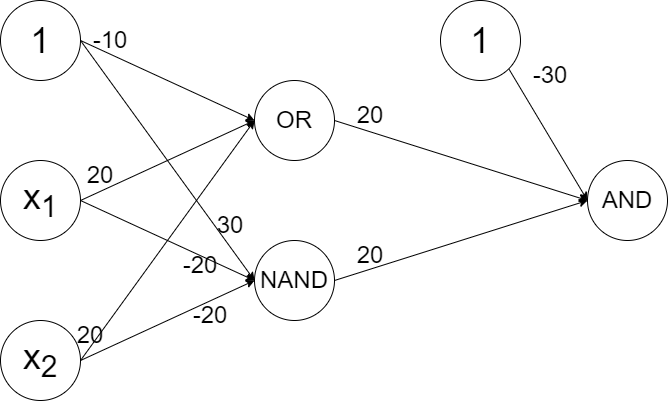
\includegraphics[width=0.6\textwidth]{figure/Xor NN.drawio.png}
  \caption{A neural network that solves the XOR problem.}
\end{figure}

\subsubsection{Backpropagation}

Since neural network introduce hidden layers, we need a new algorithm to determine how to update the weights for each layer (since no label is given for hidden layers). The backpropagation algorithm is used to update the weights of a neural network.

The core idea for backpropagation is:
\begin{equation*}
  \frac{\partial \text{Loss}}{\partial z_i} = \sum_{j \in \text{children}(i)} \frac{\partial \text{Loss}}{\partial z_j} \frac{\partial z_j}{\partial z_i}
\end{equation*}

This equation can be calculated layer by layer, starting from the output layer.

\section{Decision Trees}

A decision tree is build from top to bottom. At each step, we choose the best feature to split the data. The goal is to maximize the information gain, which is defined as:
\begin{equation*}
  \text{Information gain} = \text{Entropy}(\text{parent}) - \sum_{i} \frac{|\text{child}_i|}{|\text{parent}|} \text{Entropy}(\text{child}_i)
\end{equation*}
where $\text{Entropy}(S) = -\sum_{i} p_i \log_2 p_i$ is the entropy of a set $S$.

Noticing that the entropy of a set reaches its maximum when all classes are equally distributed, and reaches its minimum when all data points belong to the same class. The more information gain, the lower the entropy of the child nodes, the purer the child nodes.

To avoid overfitting, we can prune the tree backward. Or we can early stop the tree building process. The former is better, since we can use a validation set to determine the best time to stop.

\paragraph{CART} CART is a variant of decision tree that uses the Gini impurity to measure the impurity of a set. The Gini impurity is defined as:
\begin{equation*}
  \text{Gini impurity} = 1 - \sum_{i} p_i^2
\end{equation*}

\section{Naive Bayes}

The Naive Bayes algorithm is a simple supervised learning algorithm that is used for classification tasks. The algorithm is based on Bayes' theorem, which is defined as:
\begin{equation*}
  P(A|B) = \frac{P(B|A) P(A)}{P(B)}
\end{equation*}

The Naive Bayes algorithm assumes that the features are conditionally independent given the class label, which means we can modify the Bayes' theorem as:
\begin{equation*}
  P(y|x_1, x_2, \ldots, x_d) = \frac{P(y) P(x_1|y) P(x_2|y) \ldots P(x_d|y)}{P(x_1) P(x_2) \ldots P(x_d)}
\end{equation*}

However, this assumption is not always true. Hence, the algorithm is called "naive". Despite this, the Naive Bayes algorithm is still widely used in practice due to its simplicity and efficiency.

The Naive Bayes algorithm works as follows:
\begin{enumerate}
  \item Given a training dataset with $n$ data points and $d$ features, where the $i$-th data point is represented as $(x_{i1}, x_{i2}, \ldots, x_{id}, y_i)$, calculate the prior probability $P(y)$ and the conditional probability $P(x_j|y)$ for each feature $x_j$.
  \item For a new data point $(x_1, x_2, \ldots, x_d)$, calculate the posterior probability $P(y|x_1, x_2, \ldots, x_d)$ for each class label $y$.
\end{enumerate}

\begin{examplebox}[%
  enhanced, 
  breakable,
  skin first=enhanced,
  skin middle=enhanced,
  skin last=enhanced,
  ]{}
  For a simple 2 feature dataset with 6 data points:
  \begin{table}[H]
    \centering
    \begin{tabular}{ccc}
      \toprule
      \textbf{Feature 1} & \textbf{Feature 2} & \textbf{Class Label} \\
      \midrule
      1 & 1 & 0 \\
      1 & 0 & 1 \\
      0 & 1 & 1 \\
      0 & 1 & 0 \\
      1 & 1 & 1 \\
      1 & 0 & 1 \\
      \bottomrule
    \end{tabular}
  \end{table}

  The prior probability $P(y)$ is:
  \begin{align*}
    P(y = 0) &= \frac{2}{6} = \frac{1}{3} \\
    P(y = 1) &= \frac{4}{6} = \frac{2}{3}
  \end{align*}

  The conditional probability $P(x_j|y)$ is:
  \begin{align*}
    P(x_1 = 1|y = 0) &= \frac{1}{2} \\
    P(x_1 = 1|y = 1) &= \frac{3}{4} \\
    P(x_2 = 1|y = 0) &= 1 \\
    P(x_2 = 1|y = 1) &= \frac{1}{2}
  \end{align*}

  For a new data point $(x_1 = 1, x_2 = 1)$, the posterior probability $P(y|x_1, x_2)$ is:
  \begin{align*}
    P(y = 0|x_1 = 1, x_2 = 1) &\propto P(y = 0) P(x_1 = 1|y = 0) P(x_2 = 1|y = 0) \\
    &= \frac{1}{3} \times \frac{1}{2} \times 1 = \frac{1}{6} \\
    P(y = 1|x_1 = 1, x_2 = 1) &\propto P(y = 1) P(x_1 = 1|y = 1) P(x_2 = 1|y = 1) \\
    &= \frac{2}{3} \times \frac{3}{4} \times \frac{1}{2} = \frac{1}{4}
  \end{align*}

  Since $P(y = 1|x_1 = 1, x_2 = 1) > P(y = 0|x_1 = 1, x_2 = 1)$, the predicted class label is 1.
\end{examplebox}

\section{Ensemble Learning}

An ensemble method combines the predictions of multiple models to improve the overall performance. Some representative ensemble methods include bagging, boosting, and ramdom forest.

\subsection{Boosting}

The core idea of boosting is to train multiple weak learners sequentially, where each weak learner is trained to correct the mistakes of the previous weak learners.

Firstly, we define the error of a weak learner as:
\begin{equation*}
  \text{Error} = \sum_{i=1}^{n} w_i \mathbb{I}(y_i \neq \hat{y}_i)
\end{equation*}
where $w_i$ is the weight of the $i$-th data point, $y_i$ is the true label, $\hat{y}_i$ is the predicted label, and $\mathbb{I}(\cdot)$ is the indicator function (1 if the condition is true, 0 otherwise).

Then, we can calculate the weight of the weak learner as:
\begin{equation*}
  \text{Weight} = \frac{1}{2} \log\left(\frac{1 - \text{Error}}{\text{Error}}\right)
\end{equation*}

We the update the weight of each data point as:
\begin{equation*}
  w_i \gets w_i \exp(-\text{Weight} \times y_i \times \hat{y}_i)
\end{equation*}

The workflow of boosting is:
\begin{enumerate}
  \item Initialize the weights of the data points as $w_i = \frac{1}{n}$.
  \item For $t = 1, 2, \ldots, T$:
    \begin{enumerate}
      \item Train a weak learner $G_t$ based on the weighted data points.
      \item Calculate the error of $G_t$.
      \item Calculate the weight of $G_t$.
      \item Update the weights of the data points based on the predictions of $G_t$.
    \end{enumerate}
  \item Combine the weak learners using the weights.
\end{enumerate}

For the final prediction, we can use the weighted sum of the predictions of the weak learners:
\begin{equation*}
  \hat{y} = \text{sign}\left(\sum_{t=1}^{T} \text{Weight}_t G_t(x)\right)
\end{equation*}

\subsection{Bagging}

The core idea of bagging is to train multiple models in parallel, where each model is trained on a random subset of the data points. The final prediction is the average of the predictions of the models.

\subsection{Random Forest}

Random forest is an ensemble method that combines the ideas of bagging and decision trees. The core idea of random forest is to train multiple decision trees in parallel, where each decision tree is trained on a random subset of features.

\section{Clustering}

Clustering is an unsupervised learning algorithm that is used to group similar data points together. Some representative clustering algorithms include K-means, DBSCAN, and hierarchical clustering.

\subsection{K-Means}

The K-means algorithm is a simple clustering algorithm that is used to partition the data points into $k$ clusters. The algorithm works as follows:
\begin{enumerate}
  \item Initialize the centroids of the $k$ clusters randomly.
  \item Assign each data point to the nearest centroid.
  \item Update the centroids by taking the average of the data points in each cluster.
  \item Repeat steps 2 and 3 until the centroids converge.
\end{enumerate}

\subsubsection{How to Choose $k$} 

\paragraph{Elbow method}We can use the elbow method to determine the optimal number of clusters, which means we plot the loss function (e.g., the sum of squared errors) against the number of clusters and choose the number of clusters that corresponds to the "elbow" point.

\paragraph{G-means} G-means is a variant of K-means that uses a statistical test to determine the optimal number of clusters. The algorithm works as follows:
\begin{enumerate}
  \item Initialize $k$ as a small number.
  \item Run K-means with $k$ clusters.
  \item For each cluster, perform a statistical test to determine if the cluster fits a Gaussian distribution.
  \item If the cluster does not fit a Gaussian distribution, split the cluster into two sub-clusters.
  \item Repeat steps 2 to 4 until all clusters fit a Gaussian distribution.
\end{enumerate}

\subsubsection{How to Evaluate Clustering}

\paragraph{Internal Evaluation} Internal evaluation metrics consider the distance between data points within the same cluster and the distance between data points in different clusters. Some common internal evaluation metrics include the silhouette score and the Davies-Bouldin index.

\paragraph{External Evaluation} External evaluation metrics compare the clustering results with the ground truth labels. Some common external evaluation metrics include the adjusted Rand index and the Fowlkes-Mallows index.

\subsubsection{How to Cluster Non-Circular Data}

Use kernel K-means, which maps the data points into a higher-dimensional space where the data points are linearly separable. Other methods include spectral clustering and DBSCAN.

\subsubsection{How to Initialize Centroids}

The initialization of centroids can affect the performance of the K-means algorithm. Some common methods for initializing centroids include:
\begin{itemize}
  \item Initialize the centroids randomly.
  \item Choose each centroid furthest from the previous centroids.
  \item Try multiple initializations and choose the one with the lowest loss.
\end{itemize}


\end{document}	